\section{8.38}
\subsection{a)}

\paragraph{Specification:}
2 forces $\vec{F_1}$ and $\vec{F_2}$ are effecting the same point $P$. 

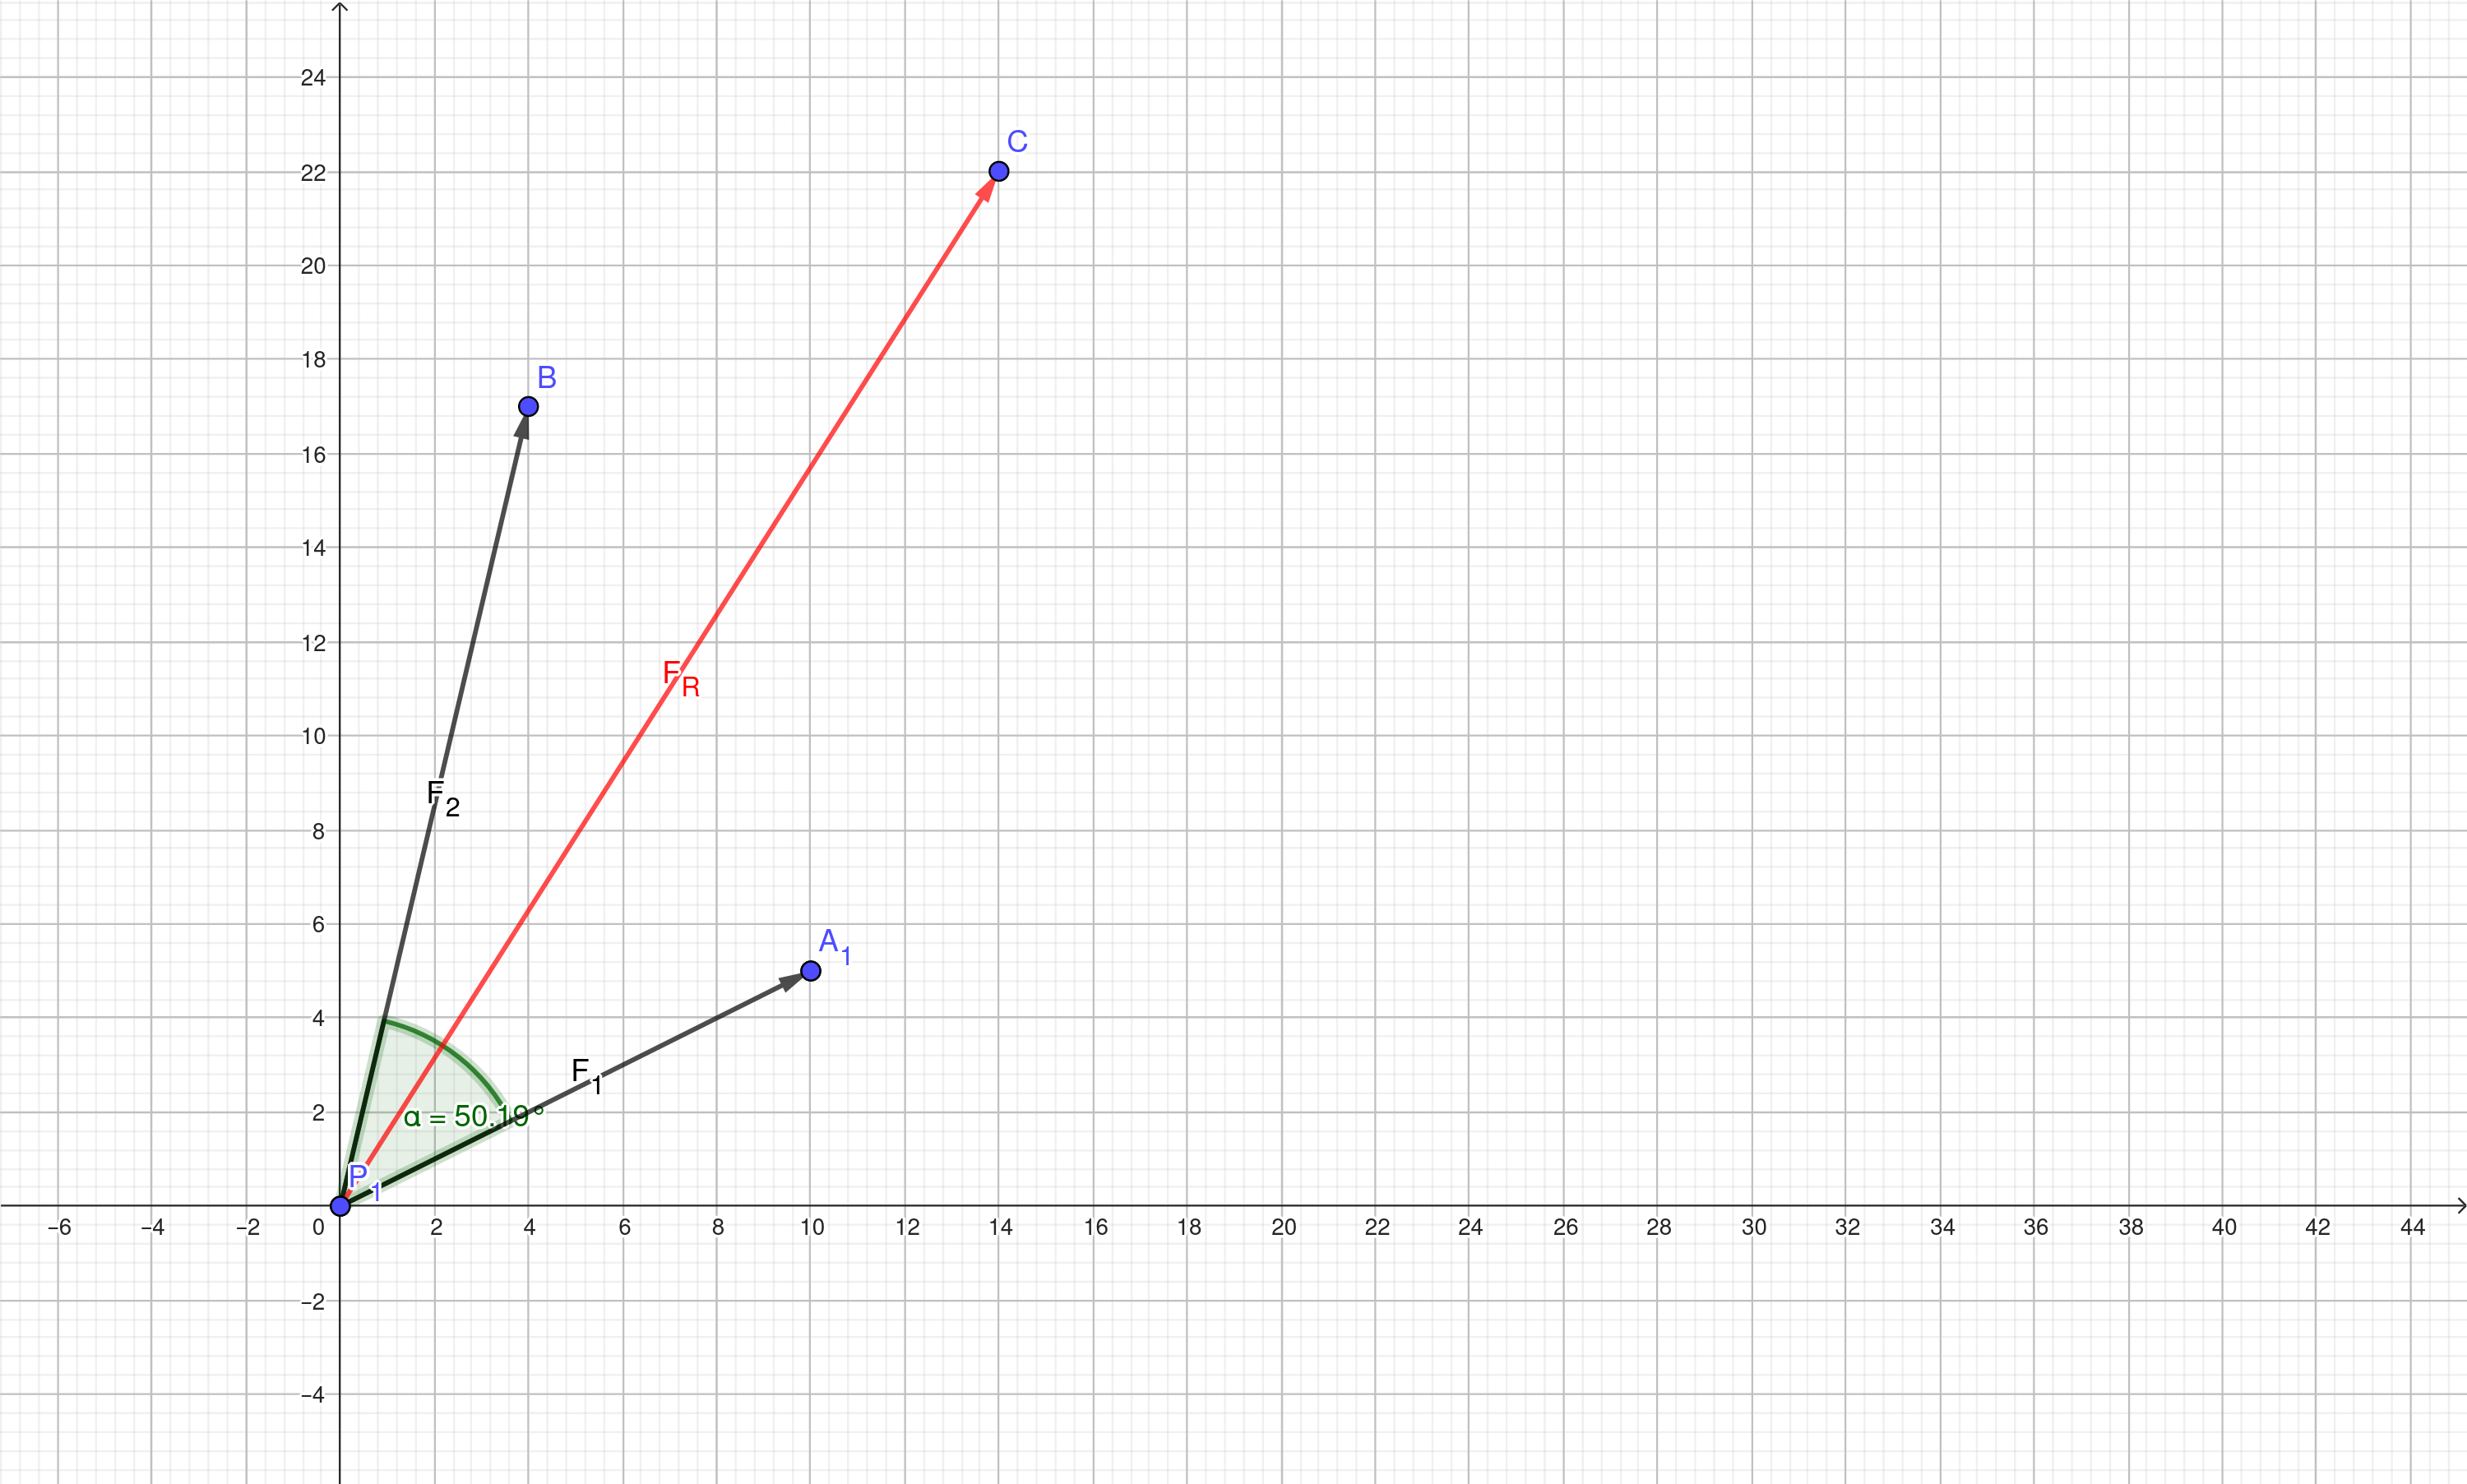
\includegraphics[width=\linewidth]{images/8-38.png}

\paragraph{Requirements:}
Calculate the resulting force $\vec{F_R}$ and the angle $\phi$ between $\vec{F_1}$ and $\vec{F_2}$ 
(unit = Newton).

\def\vFOne{\begin{pmatrix}
       10 \\ 
       5
    \end{pmatrix}}

\def\vFTwo{\begin{pmatrix}
       4 \\ 
       17
    \end{pmatrix}}

\def\vFR{\begin{pmatrix}
       14 \\ 
       22
    \end{pmatrix}}

\paragraph{Definitions:}
\begin{align}
    \vec{F_1} &= \vFOne \\
    \vec{F_2} &= \vFTwo
\end{align}

\paragraph{Exercises:}
\begin{align}
   \vec{F_R} &= \vec{F_1} + \vec{F_2}  \\
   \vec{F_R} &= \vFOne + \vFTwo \\
   \vec{F_R} &= \vFR \\
   |\vec{F_R}| &= \sqrt{14^2 + 22^2} \\
   |\vec{F_R}| &= 26.0768096208 \\[20pt]
   \cos(\phi) &= \frac{\vec{F_1} \cdot \vec{F_2}}{|\vec{F_1}| * |\vec{F_2}|} \\
   \cos(\phi) &= \frac{\vFOne \cdot \vFTwo}{\sqrt{125} * \sqrt{305}} \\
   \cos(\phi) &= \frac{125}{195.256241898} \\
   \phi &= \arccos(0.640184399663) \\
   \phi &= 50.19443^\circ
\end{align}

\paragraph{Answer:}
The resulting force $F_R$ has a magnitude of 26.0768096208 Newton and the angle $\phi$ between the forces 
$\vec{F_1}$ and $\vec{F_2}$ is 50.19443$^\circ$.
